\section{Experimental Study}\label{sec:expr}

To evaluate the performance of backbone computing, we compare \tool with state-of-art backbone computing tool \minibones. We choose total solving time as our main matrix. In the experiments, SAT testing is the take the major part of solving time, different formula requires different numbers of SAT testings. We choose the number of SAT testings as another matrix. Unlike the previous in \cite{JLM15}, that only compare the total solving time of each formula, we separate formulae into groups. For example, if a set of formulae are generated from hardware model checking problem, then they are in the same group. We study performance of \tool in different groups, results show that \tool outperforms \minibones in $\textit{manthey}$ group, saving 34\% of solving time.

\subsection{Benchmark Setup}
We implemented our approach in a tool called \tool written in C++ interfacing MINISAT 2.2 \cite{MINISAT}.
% It's available at xxx.
There are 3 industrial benchmarks, consists of 72 industrial satisfiable formulae and 86 random benchmark, consisted 6606 generated satisfiable formulae. Each formula in an industrial benchmark is selected from verification of the same application, each formula in a random benchmark are generated from the same unsatisfiable formula. Formulae in the same benchmark share some common features, such as the number of variables and clauses, the structure of the formula and so on.

The experiments were conducted on a cluster of IBM iDataPlex 2.83 GHz, each industrial formula was running with a timeout of 1800s and memory limit of 4GB. Each random formula was running with a timeout of 100s and memory limit of 256 MB. Our experiments benefit from the small scale of generated formulae, which allow us to run more formulae at the same time.

We select 72 industrial formulae from SAT competitions, 34 are them are solved by both \tool and \minibones. We also select 100 crafted formulae from SAT competitions, none of them are solved within time and memory limits. Although MINISAT is not designed to solve random formulae, but both \tool and \minibones use MINISAT as their SAT solvers, we consider it fair to use random formulae to test the scalability of \tool. Instead of directly using satisfiable random formulae from SAT competitions, we generate 6606 satisfiable formulae from unsatisfiable formulae. Satisfiable random formulae in SAT competitions have different features and adjacent structures. Generated formulae from the same unsatisfiable formula share similar community structure from nature. We would like to explore the relationship between features of structures of the formula and the performance of \tool. Another reason is that, unlike other random formula that requires more than 500 seconds solving time, the solving time of generated formula range from 1 seconds to 100 seconds, which saved lots of solving time and make our experiments more practicable.

There are 3 benchmarks among industrial formulae, which are $\textit{mrpp}$, $\textit{manthey}$ and $\textit{dimacs}$. The comparison between \tool and \minibones are analyzed in different benchmarks.
For generated formulae, they are grouped into 86 benchmark since there are 86 different formulae that generate them.

We separate formulae into different benchmarks to study the effects of different adjacent structures on the performance of \tool. Adjacent structures are presented as adjacent graph of a formula. The nodes in the graph stands for variables, if two variables shared the same clause, there is an edge between them. In the graph, the more adjacent variables a variable has, the more center the variable located. In the middle of an adjacent graph, there is a ball-like core formed by variables that has multiple neighbours, if a variable has less neighbours, it will locate apart from the core, the less neighbours a variable has, the farer it located to the core.

\subsection{Experimental Results on Industrial Formulae}\label{sec:ind_expr}
Among the 72 industrial formulae, both \tool and \minibones are able to solve 34 of them.
The details of solving time and SAT tests number comparison of each benchmark are shown in Table \ref{tab:ind}, we use $st$ to denote the solving time of each tool and $sc$ to denoted the SAT tests number of each tool. We can observe that \tool saved 38\% solving time compared to \minibones in $\textit{manthey}$ benchmark, with 17\% saving on SAT tests numbers. In $\textit{mrpp}$ benchmark, \minibones saved 3\% solving time and 23\% SAT tests number respectively. In total, \tool saved 27\% solving time and 4\% less SAT calls. Our experiments result prove the observation in \cite{JLM15} that less SAT calls will lead to a faster solving.
Figure \ref{fig:ind} shows the solving time of all 34 industrial formulae, there are only 4 formulae that \minibones outperforms \tool.
\begin{table}[t]
\centering
\begin{tabular}{ccccccc}
\toprule
 Benchmark &st of \tool(s) &st of \minibones (s) & st Difference (\%) &sc of \tool &sc of \minibones \\
\midrule
mrpp & 3945 & 3792 & 3 & 28261 & 21555 \\
manthey & 2935 & 4810 & 38 & 49356 & 59562 \\
dimacs & 1339 & 1369 & 2 & 2018 & 2022 \\
total & 7219 & 9971 & 27 & 79635 & 82139 \\

\bottomrule
\end{tabular}
\caption{Solving Time and SAT Tests Number Comparison on Industrial Formulae}
\label{tab:ind}
\end{table}


\begin{figure}
    \centering
    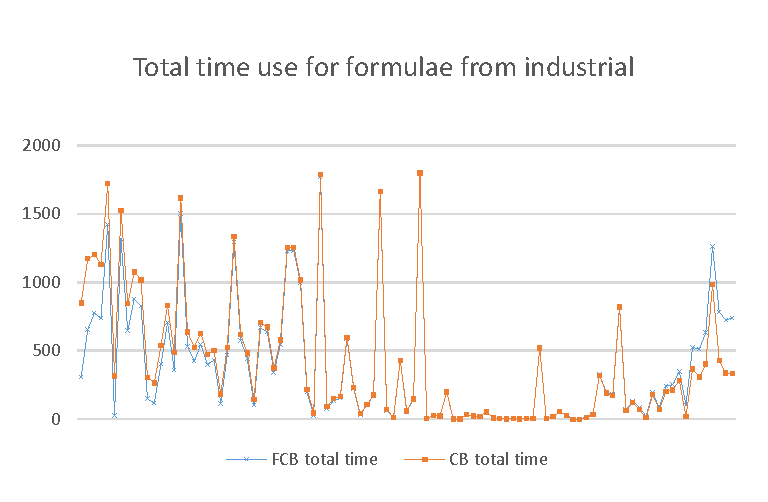
\includegraphics[scale=0.3]{ind.pdf}
   \caption{Solving Time Comparison on Industrial Formulae}
   \label{fig:ind-time}
\end{figure}


In order to dig the underlying reason that why \tool outperforms \minibones in $\textit{manthey}$ benchmark, we consider the structure feature of the given formula. Formulae in the same benchmark share common feature in the structure, it's because that a specific application always has its own pattern when encoded into satisfiable problem. We explore the adjacent structure of the formulae in a given benchmark, we found that $\textit{manthey}$ have a star-like adjacent structure as shown in \ref{fig:star}. It means that variables in the given formula in $\textit{manthey}$ are separated into several groups. Inside the groups, variables are connected tightly, perhaps one variable is adjacent to every other variable in the group. Connections between groups are loosen, only a few variables adjacent to another variable outside the group. Experiments show that \tool performs better on the star-like formula.
\begin{figure}
\centering 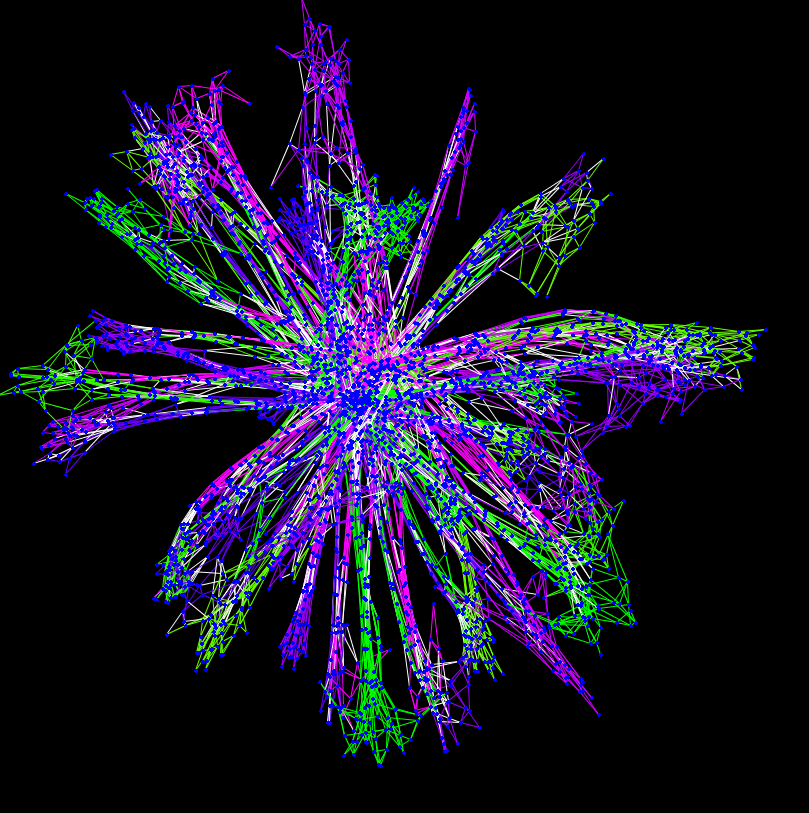
\includegraphics[scale=0.3]{star.png}
\caption{Adjacent Structure of manthey}\label{fig:star}
\end{figure}

On the other hand, the adjacent structure of formulae in $\textit{mrpp}$ are more like a football as shown in \ref{fig:ball}. All variables have a large amount of adjacent variables, and they are almost connected to each other. It's hard to find a variable that only has a few adjacent variables. However, there are 2 special formula in $\textit{mrpp}$ that has several group of variables that are less connected as shown in \ref{fig:mrpp_s}, it looks like there are several by-passes around the center core. experiments show that, \tool outperforms \minibones on these 2 formula.
\begin{figure}
\centering 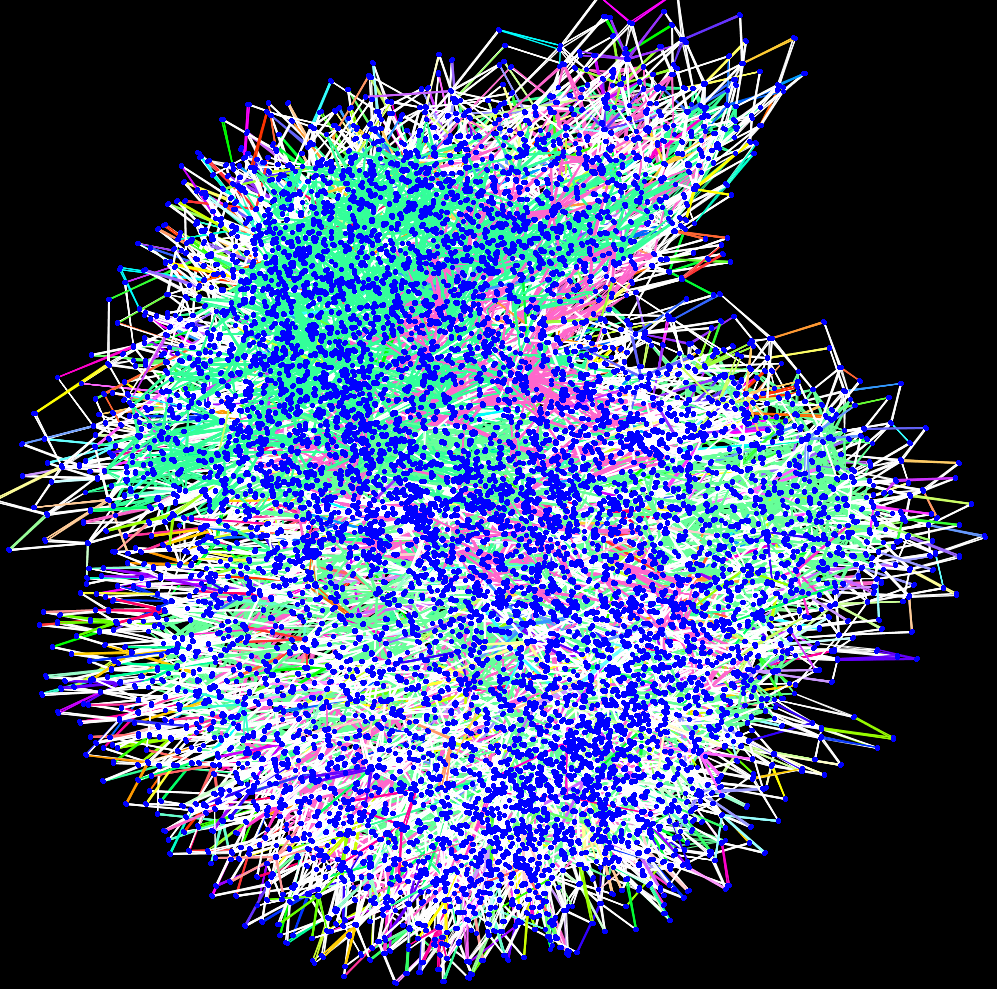
\includegraphics[scale=0.3]{ball.png}
\caption{Adjacent Structure of mrpp}\label{fig:mrpp}
\end{figure}
\begin{figure}
\centering 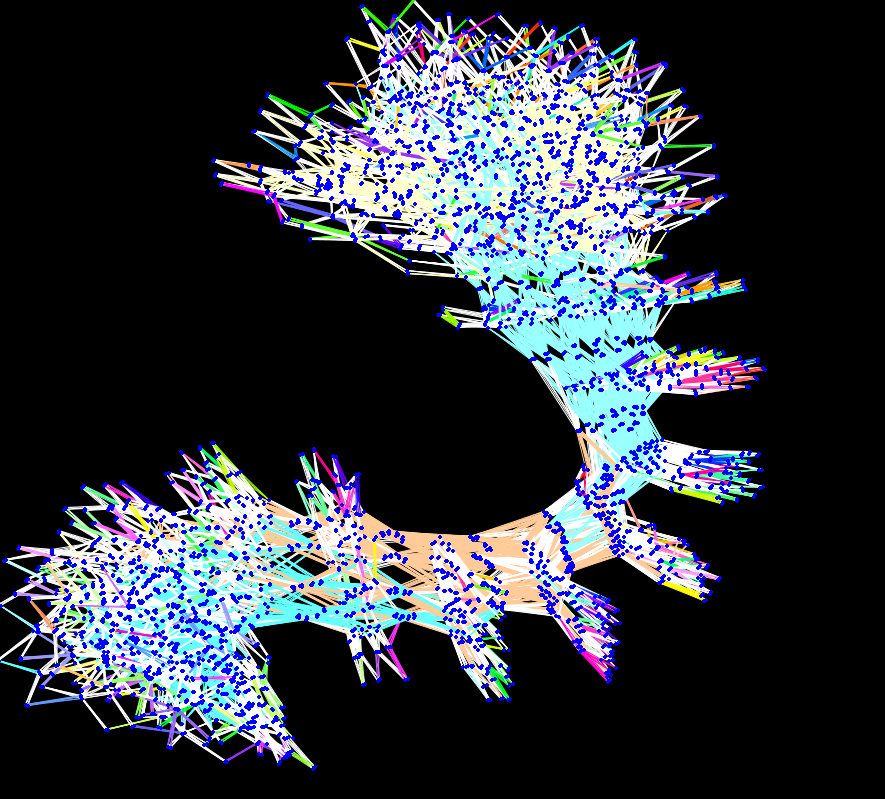
\includegraphics[scale=0.3]{mrpp_s.png}
\caption{Adjacent Structure of special mrpp}\label{fig:mrpp_s}
\end{figure}

Based on the observation, we concluded that \tool is better at solving formula that variables can be separated into less connected groups, such a star adjacent structure or a structure with a center and several branches or by-passes.


SAT solving time and SAT calls of different benchmark, only with Algorithm 1.
The same table and analysis for Algorithm 2. a table with 1, 2, 1+2.
A general comparison result about Algorithm 1 and Algorithm 2.
The results show that for formulae in $\textit{manthey}$, the combination is the best. The contribution is almost the same.
For $\textit{mrpp}$, the combination is not the best solution, this explains why our algorithm performs poorly on this benchmark, one step of the computing doesn't behaves well. It's because that the formula in this benchmark are hard to test whether a literal is a backbone,(seen the gap between the first model solving time and the total solving time). The reason for this is because the variables here shared a very tight relations, it will causes lots of conflicts by any wrong decision.

For industrial formulae, both \tool and \minibones are able to solve 34 formulae out of 72. For generated formulae, both \tool and \minibones are able to solve the total 6606 formulae under time and memory limits.
Experiments show that for \textit{mrpp} benchmark, \minibones solved 4\% times faster, and for $\textit{manthey}$ benchmark, \tool reduces 38\% solving time. \tool reduces 2183 seconds of solving time of industrial formulae, saving 21\% solving time in total.

When we take a close look at the formulae that are accelerated by \tool from industrial benchmark, we found that the adjacent structure of these formulae shared some common features. Experiments show that different formula has different structures, formulae from the same benchmark often have similar structures. Compared with the ball-like structure for formulae in $\textit{mrpp}$, formulae in $\textit{manthey}$ benchmark have more star-like structures. There are two formulae in $\textit{mrpp}$ that have a pipe-like structure, where there are several branches near the main root-like core, \tool performs better on this two formula.


\subsection{Results for Generated Formulae}
How many solving time saved in total, what proportion.
Show the total solving time and SAT calls of selected 3 benchmark, accelerating 1, the same 1, decline 1.
Show the statistic results of different benchmarks, how many accelerating, more than how large proportion, how many the same, how many decline, at how large proportion

Explain the relation between adjacent structure and performance.
3 pictures

Based on this observation, we divide 6606 random formulae into three groups according to their community structures.
The \emph{simple group} contains 371 formulae whose community structures are divergent,
the \emph{hard group} contains 337 formulae whose community structures are focusing,
and the \emph{medium} group contains 5898 formulae between divergent and focusing.


Table \ref{tab:mcs-graph} shows the experiments results on these three groups. \textit{cb100} performs better than \tool on the simple group, as \textit{cb100} tries to find a backbone literal by complementing models as soon as possible, which are the vertexes far from the center.
\tool outperforms \textit{cb100} for both medium group and hard group.
\tool reduces by 8\% for medium group and by 40\% for hard group of the total running time.

The experimental results show that \tool performs better than \textit{cb100} on hard random formulae and is comparable to \textit{cb100} on simple formulae.

NOTE: draw the community structure of the unsatisfiable formula
For formulae generated from an unsatisfiable formula with a very sharp community structure, that is there is exactly one obvious edge that sperate away from the core of variables, \tool performs quite well, almost needs less than 5 seconds to compute backbone.
For formulae generated from an unsatisfiable formula with a ball-like structure, both \tool and \minibones need almost more than 20 seconds to solve. This indicates that ball-like structure are hard to complex backbone. If we compare the solving time of first model between type I and type II, we can find that it's more changeling for MINISAT to solve type II, because there is no short-cut to find a good assignment quickly.
For the rest of formula, a core with multiple branches around the core, \tool performs better than \minibones on most of the generated formulae.


\begin{figure}
\centering 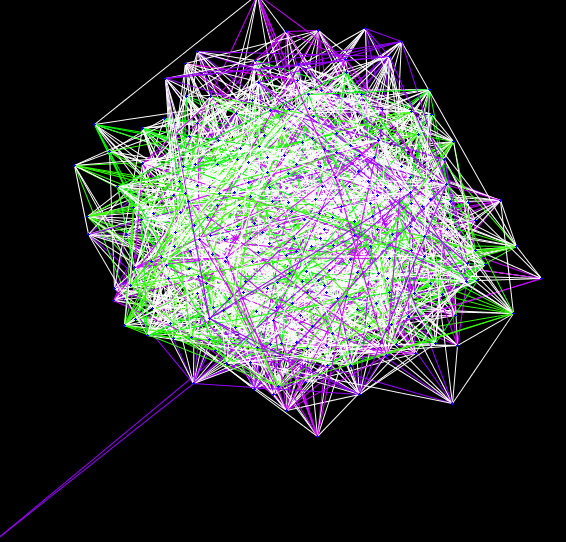
\includegraphics[scale=0.3]{uuf250-090.png}
\caption{}\label{}
\end{figure}
\begin{figure}
\centering 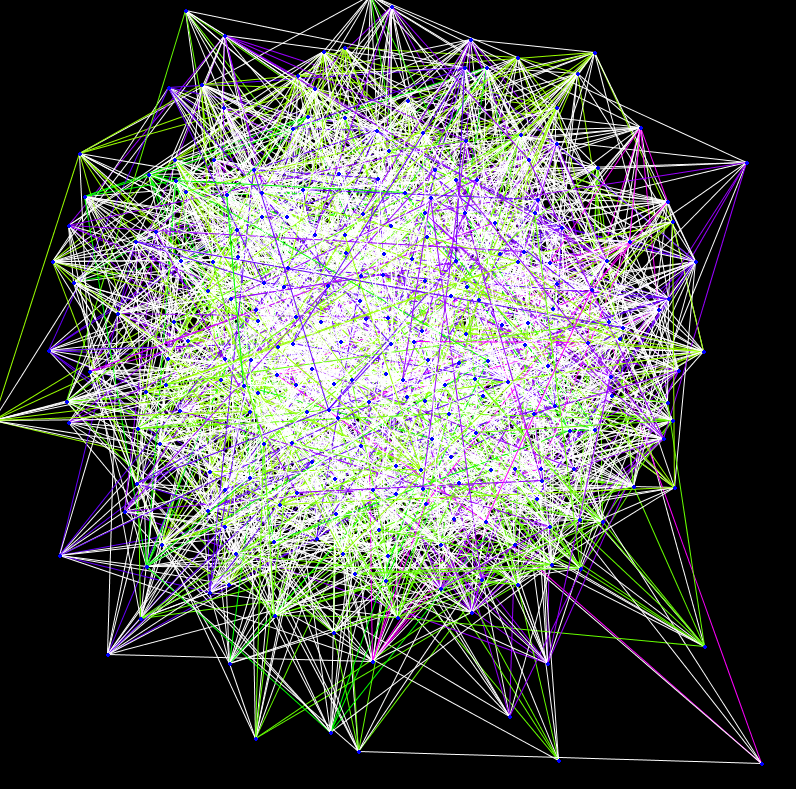
\includegraphics[scale=0.3]{uuf070.png}
\caption{}\label{}
\end{figure}
\begin{figure}
\centering 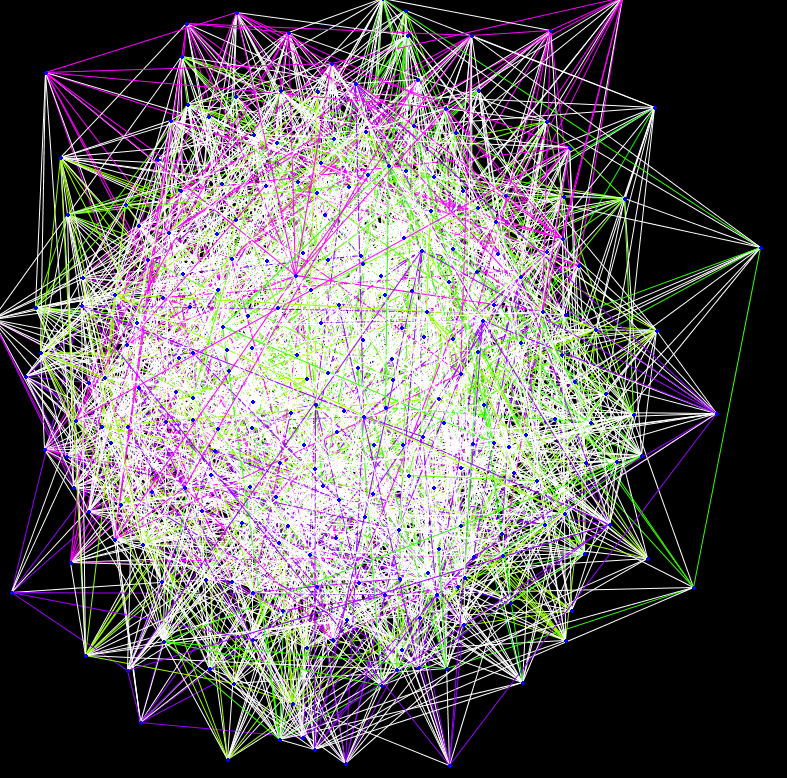
\includegraphics[scale=0.3]{uuf030.png}
\caption{}\label{}
\end{figure}



